% Chapter 3

\chapter{LHC} % Main chapter title

\label{ch:LHC} % For referencing the chapter elsewhere, use \ref{Chapter1} 

\lhead{Chapter 3. \emph{LHC}} % This is for the header on each page - perhaps a shortened title

%----------------------------------------------------------------------------------------
The Large Hadron Collider (LHC) at CERN is a wonder of engineering and technology. It lies inside a 26.7 Km circular tunnel and 100 meters under the ground. Its construction took over 15 years, involved engineers from all over the world and costed over 6.5 billion CHF. Inside the tunnel there are two counter-rotating hadron beams accelerated to energies up to 7 TeV each. This beams are then forced to collide inside four huge detectors that measures the products of the collision\citep{LHCMT}.
\section{Characteristics}
The 26,659 m tunnel used by the LHC was inherited from the LEP, when it was shut down. The basic layout consists of eight long straight sections and eight bending arcs\citep{keil}. In order to keep the 7 TeV proton beams in such a small orbit it was necessary to use 1,232 magnets with a 8.3 T field that extend to a length of 14.3 m each\citep{DR}. To achieve this, powerful magnetic field superconducting magnets were to be used. Because of commercial availability NbTi superconductors were used, this material needs to be cooled down below 4.2 K to reach the superconducting state.
The solution was, and still is, to keep the magnets submerged in superfluid Helium below 2 K\citep{keil}.
The basic layout is shown in Figure \ref{Schem}, where Beam 1 is shown in blue and circulates clockwise; and in red Beam 2 which  rotates counterclockwise. There are four intersections, one in each major experiment: ATLAS, CMS, LHC-b, and ALICE. The first two, ATLAS and CMS, are high luminosity experiments and are located diametrically opposite to each other, while LHC-b is an devoted to quark b experiments, and ALICE stands for A Large Ion Collider Experiment, which is self-explanatory and work with full stripped Pb ions. The LHC consist of 8 arcs and 8 straight section and it is divided in octants, that start at the center of on arc and end at the center of the next one\citep{DR}. 
\begin{figure}
	\centering
  \begin{minipage}{\textwidth}
  	\centering
   	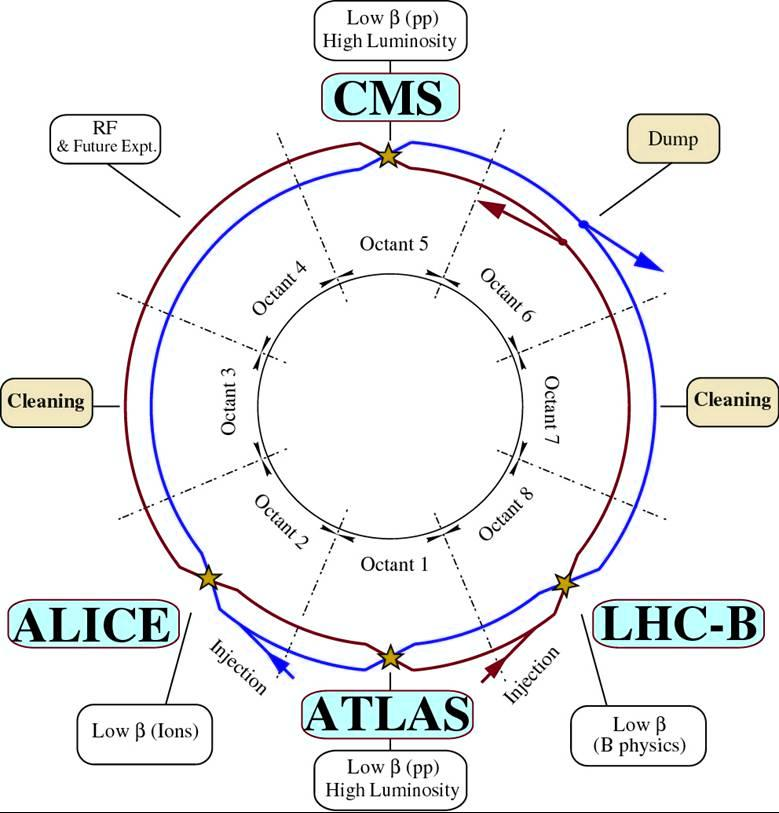
\includegraphics[width=3.5in]{Pictures/imagen.jpg}
  		\caption{\label{Schem}
   			General schematic for the LHC}
   			\footnotesize{Picture courtesy of CERN.}
   \end{minipage}
\end{figure}
The main parameters when working at its maximum energy are listed in Table \ref{table:LHCparam}. 
\begin{table}%[ht]
%\centering % used for centering table
\caption{Main parameters for proton-proton collisions} % title of Table
\begin{minipage}{\textwidth}
\renewcommand{\thefootnote}{\thempfootnote}

%\footnote{This table was taken from "the LHC vacuum system", p. 292 \citep{vacuum}. }
\begin{tabular}{l c}% centered columns (4 columns)
\hline
Energy \hspace{8.5cm} & 7 TeV \\ % inserting body of the table
Dipole Field & 8.33 T \\
coild aperture & 56 mm \\
Luminosity &10\textsuperscript{34} s\textsuperscript{$-$1} cm\textsuperscript{$-$2} \\
Injection energy & 450 GeV \\
Circulating current/beam & 0.56 A\\
Bunch spacing & 25 ns \\
Particles/bunch & 1.1$\times$10\textsuperscript{11} \\
Stored beam energy & 350 MJ \\
Normalised trasverse emittance & 3.75 $\mu$m \\
RMS bunch length & 0.075 m \\
Beam lifetime & 22 h \\
Luminosity lifetime & 10 h \\
Energy loss/turn & 6.7 keV \\
Critical photon energy & 45 eV \\
Linear photon flux & 1$\times$10\textsuperscript{17} m\textsuperscript{$-$1}s\textsuperscript{$-$1} \\
Total radiated power/beam & 3.8 kW \\ [1ex] % [1ex] adds vertical space
\hline
\end{tabular}
\end{minipage}
\begin{minipage}{\textwidth}
\begin{footnotesize}
* This table was taken from "the LHC vacuum system", p. 292 \citep{vacuum}.
\end{footnotesize}
\end{minipage}
\label{table:LHCparam} % is used to refer this table in the text
\end{table}

\subsection{Arc Cells}
The arcs consist of 23 regular arc cells. These are made out of two 53.45 m long half cells each of which consist of one cold mass with a length of 5.355m (6.63 mlong cryostat) short straight section (SSS) assembly and three 14.3 m long dipole magnets. The optics of Beam 1 and Beam 2 are coupled by electrical connections of the main magnets. There is also a dispersion suppressor at every transition between arcs and straight sections. The arc cells emulate a FODO lattice\citep{DR}.
\subsection{Optics}
The LHC optics design allows an optics matching with fixed and equal phase advances over the insertion regions for both beams that does not perturb the optics in the rest of the machine. The total number of particle trajectory oscillations during one revolution in the storage ring of the machine is adjusted by the optics of the arc cell. The flexibility of the phase advance over the insertions provides a measure for the flexibility of the total LHC optics and tell us how much liberty we have to change the phase advance between the main experimental insertions\cite{DR}.

\subsection{LHC Beam Pipe}
Because of the high beam intensities given by luminosities such as the one shown in Table \ref{table:LHCparam}, the LHC cannot work the same way as the Tevatron, which uses a single vacuum chamber and one set of magnets for both beams, the LHC requieres a vacuum chamber and set of magnets for each beam, and the beams only share the regions where the collisions take place and are around 130 m long\citep{DR}.
On one hand we have the price of the magnets and on the other hand we have the problem that there is not enough space in the LEP tunnel for two sets of magnets; as a result the LHC was built with twin bore magnets constructed of two sets of coils and beam channels within the same mechanical structure and cryostat\citep{DR}.

\textcolor{black}{90\% of the LHC surface should be maintained below 20 K and is made of copper cladded stainless steel in order to reduce ohmic resistence. The rest can stay at room temperature and is made of thick copper beam pipe \citep{DR}.}


\label{screen}
Another important feature of the beam pipe is the beam screen, this is a cooled screen intended to intercept SR at temperatures higher than 1.9 K and electrons due to electron clouds in order to prevent the magnets from heating. Figure \ref{fig:screen} shows the conceptual design of the LHC beam screen\citep{DR}\citep{vacuum}. 
\textcolor{black}{
The manufacturing process starts by co-laminating a specially developed low permeability 1mm thick
austenitic stainless steel strip with a 75 $\mu$m copper sheet and rolling a saw-tooth structure which  will intercept photons at normal incidence, thereby reducing the amount of reflected photons. The pumping slots are punched into this composite strip, which is then rolled into its final shape and closed by a longitudinal
weld\citep{vacuum}.
}
\begin{figure}
	\centering
  \begin{minipage}{\textwidth}
  	\centering
   	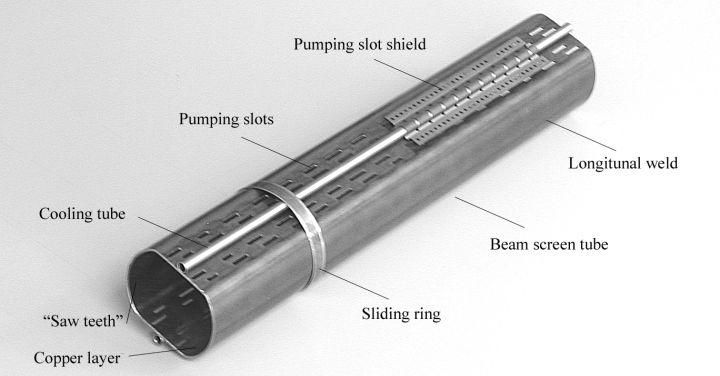
\includegraphics[width=3.5in]{Pictures/screen.png}
  		\caption{\label{fig:screen}
   			LHC Beam Screen}
   			\footnotesize{Picture courtesy of CERN.}
   \end{minipage}
\end{figure}

\subsection{Cryogenics}
\label{cryo}
The LHC uses cryomodules that consume liquid helium and expel evaporated helium. Each module looses 150 W statically in addition to the dynamic losses, that span from 100 W to 800 W.
For operation at nominal field the pressure inside the helium tank has to be carefully controlled to avoid frequency variations of the cavity\citep{DR}.
\subsection{Synchrotron Radiation}
The LHC is the first proton collider for which SR is a problem. At its highest energies SR gives rise to an important heat load to the beam screen\citep{DR}, mentioned in \ref{screen}. As shown in Table \ref{table:LHCSR} each beam produce an average of 6.8 $\times$ 10\textsuperscript{16} photons per metre per second in the arcs, which corresponds to 3886 W. So the SR power per metre per bend per beam is 220 mW/m. 

\begin{table}%[ht]
\caption{SR Parameters} % title of Table
%\centering % used for centering table
\begin{minipage}{\textwidth}
\begin{tabular}{l c c}% centered columns (4 columns)
\hline
\hline %inserts double horizontal lines
Parameter & 450 Mev & 7 TeV \\[0.5ex]% inserts table heading
\hline % inserts single horizontal line
Total power/beam & 0.066 W & 3886 W \\ % inserting body of the table
Energy loss per turn & 0.11 eV & 6.7 keV \\
average photon flux per metre and second & 0.4 $\times$ 10\textsuperscript{16} & 6.8 $\times$ 10\textsuperscript{16} \\
Photon critical energy & 0.01 eV & 43.13 eV \\
Longit. emittance damping time & 5.5 yr & 12.9 h \\
Trans. emittance damping time & 11 yr & 26 h \\ [1ex] % [1ex] adds vertical space
\hline %inserts single line
\end{tabular}
\end{minipage}
\begin{minipage}{\textwidth}
\begin{footnotesize}
* This table was taken from the "LHC Design Report", p. 108 \citep{DR}.
\end{footnotesize}
\end{minipage}
\label{table:LHCSR} % is used to refer this table in the text
\end{table}

%----------------------------------------------------------------------------------------


\section{Electron Cloud Due to Beam Induced SR}

When high energy SR photons strike a surface, they are able to set loose electrons out of the surface by ionizing it. This electrons are then attracted by the protons in the beam, they move, hitting the wall extracting even more electrons out of the wall, that will follow the next bunch of protons, this process leads to a fast building electron cloud, which is a very undesirable effect. The effects of electron clouds have been studied at CERN since 1997\cite{rumolo2011electron}.


%\subsection{Sawtooth Pattern}
%----------------------------------------------------------------------------------------


